\section{Постановка задачи и основные соотношения}
%Будем рассматривать рассеяние плоской электромагнитной волны на рассеивателях в различных диапазонах частот для шариков, состоящих из серебра, меди и золота. Представим шарики ввиде сфер и рассмотрим три случая, для одиночной сферы Рис.\ref{fig:1st_scatterer}, для 5 сфер Рис.\ref{fig:2nd_scatterer} и для 17 сфер Рис.\ref{fig:3td_scatterer}. Однако пред этим, найдем рассеянние на цилиндре численным и точным методом решения, чтобы убедиться в правильности получаемых данных. \\
Будем рассматривать рассеяние плоской монохроматической электромагнитной волны на рассеивателях различной геометрии в широком диапозоне частот. Поле такой электромагнитной волны описывается следующим образом
\begin{align}
	&\vec{E}= \vec{x}_0{E}_{0} \exp (i\omega t - i k_0z)\\
	&\vec{H}= \vec{y}_0{E}_{0} \exp (i\omega t - i k_0z)
\end{align}
В качестве рассеивателей будет рассматриваться несколько самоподобных (фрактальных) объектов увеличивающейся сложности. Так, на <<нулевой>> итерации рассеиватель --- это просто однородный шар (см. Рис. \ref{fig:1st_scatterer}); на второй --- пять шаров (см. Рис.\ref{fig:2nd_scatterer}), наибольший из которых совпадает с шаром на предыдущей итерации, а 4 малых шара имеют радиусы в 2 раза меньше радиуса большой сферы; на третьей итерации --- 17 шаров (см. Рис. \ref{fig:3td_scatterer}), самые малые шары имеют радиусы в 2 раза меньше, чем радиусы малых шаров на предыдущей итерации. Все центры шаров располагаются в плоскости $xOy$. Материалы всех элементов, составляющих рассеиватели считаем одинаковыми. В качестве вещества, заполняющего шары, будем рассматривать серебро, медь и золото. Ввиду хорошей проводимости этих веществ на низких частотах элементы рассеивателей могут быть заменены тонкостенными сферами, из-за присутствия скин--эффекта в этих диапазонах длин волн.
\newpage
\begin{figure}[h!]
	\centering
	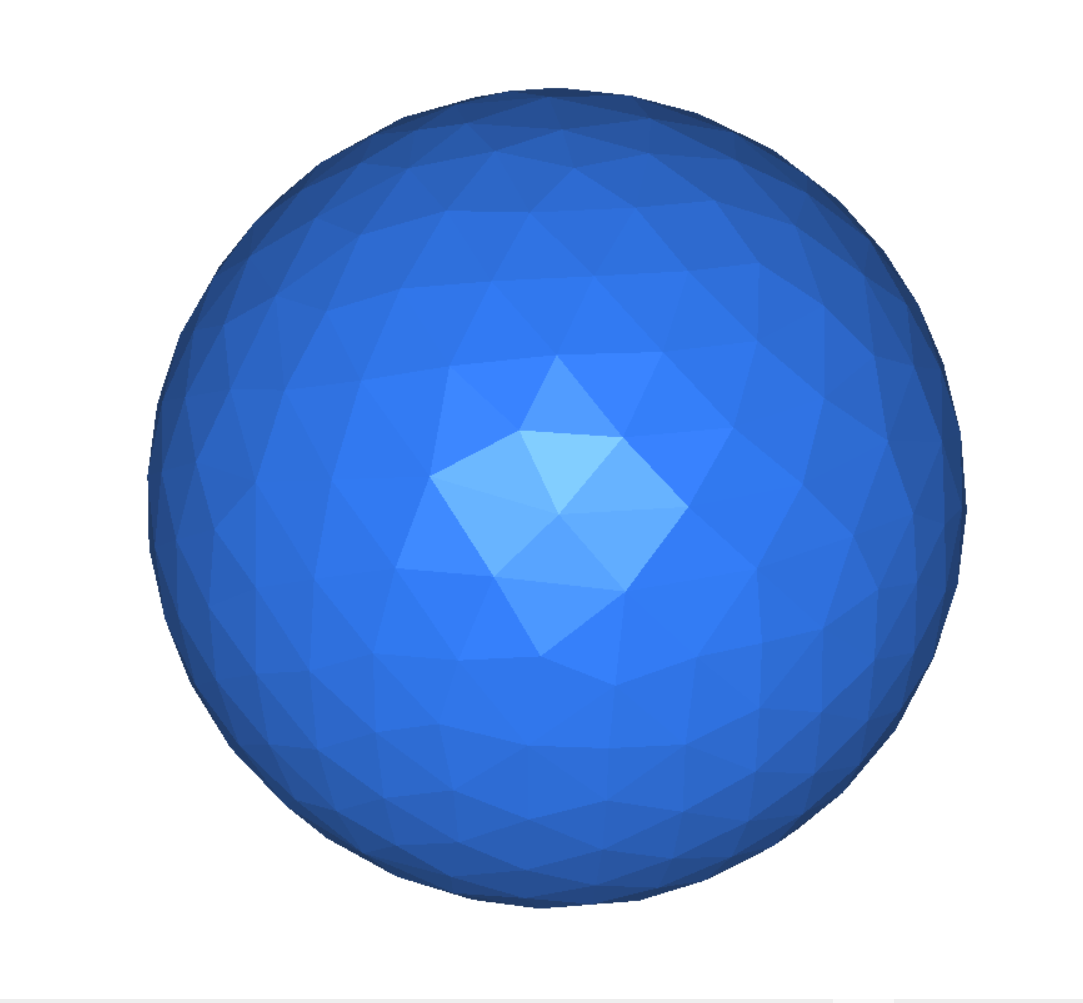
\includegraphics[width=0.4\linewidth]{1st_scatterer}
	\caption{Единичная сфера}
	\label{fig:1st_scatterer}
\end{figure}
\begin{figure}[h!]
	\centering
	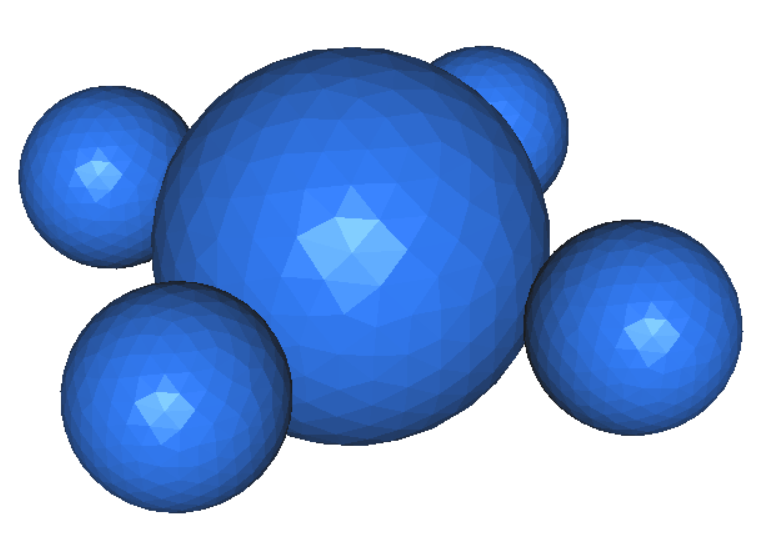
\includegraphics[width=0.5\linewidth]{2nd_scatterer}
	\caption{Первая итерация - 5 сфер}
	\label{fig:2nd_scatterer}
\end{figure}
\begin{figure}[h!]
	\centering
	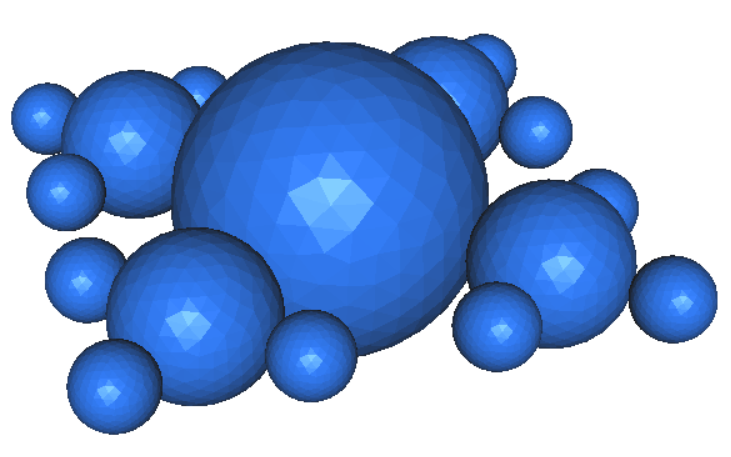
\includegraphics[width=0.5\linewidth]{3td_scatterer}
	\caption{Вторая итерация - 17 сфер}
	\label{fig:3td_scatterer}
\end{figure} 
\section{Описание метода решения задачи}
Запишем уравнения Максвелла:
\begin{align}
 {\rm rot}\vec{E} &= -\dfrac{1}{c}\dfrac{\partial \vec{B}}{\partial t} \\
 \rm rot\vec{H} &=\dfrac{4\pi}{c}\vec{j} + \dfrac{1}{c}\dfrac{\partial \vec{D}}{\partial t} \\
 \rm div\vec{D} &= 4\pi \rho \\
 \rm div\vec{B} &= 0 
\end{align}
При этом не забыв про материальные уравнения, описывающие характеристики среды, в которой распространяется электромагнитная волна:
\begin{align}
	   \vec{D} &= \varepsilon \vec{E}\\
	   \vec{B} &= \mu \vec{H} \\
	   \vec{j} &= \gamma \vec{E}
\end{align}
Решим задачу дифракции одиночной сферы используя метод конечных элементов. Для этого наш объект заключим в сферическую область, в которой будут рассеиваться волны. Сразу определим, что внутри нашего объекта область заполнена диэлектриком, а его радиус будет в 10 раз меньше длины волны принимаемой для расчетов ($ \lambda = 1 $), а радиус сферической области в 4 раза больше (Рис.\ref{fig:ces1}). Так же стоит отметить, что на протяжении всей работы будет использоваться гармоническая зависимость $ e^{j \omega t} $, где $ j = \sqrt{-1} $. Далее найдем сечение рассеяния $ \sigma_s $ и сечение поглощения $ \sigma_a $, которое будет находиться на удалении $ \lambda = 3 $, с помощью действительной $ \varepsilon' $ и мнимой $ \varepsilon'' $ части диэлектрической проницаемости на основе коэффициентов преломления $ n' $ и $ n'' $. Сделаем тоже самое для всех трех случаев.  Для удобства поиска решения расчеты будем производить в декартовой системе координат. \\
\begin{figure}[h!]
	\centering
	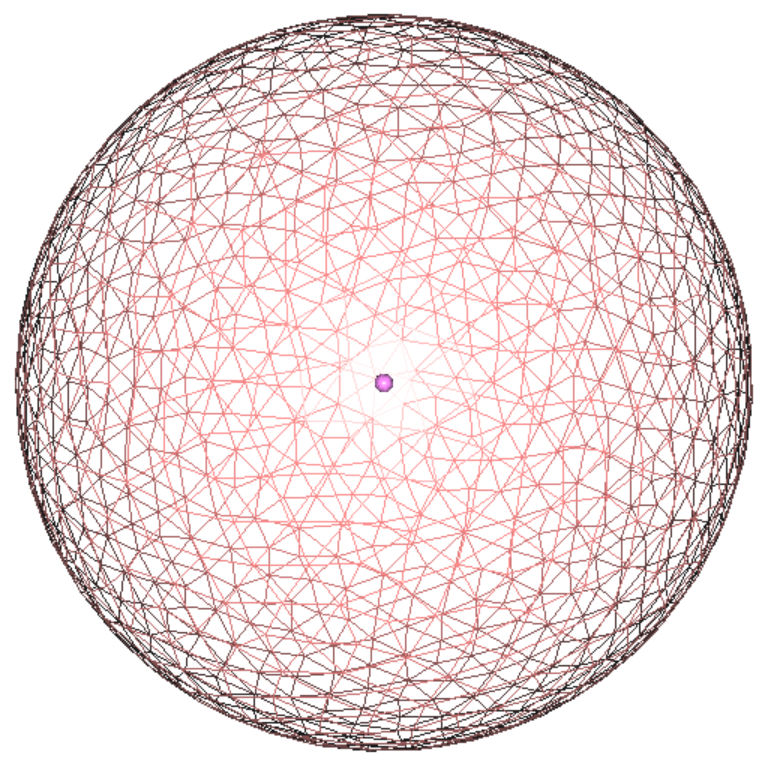
\includegraphics[width=0.4\linewidth]{ces1}
	\caption{}
	\label{fig:ces1}
\end{figure} \\
На Рис.~\ref{fig:3td_scattererAndOuterSpheres} можно увидеть случай с 17 сферами, где в центре находится сам объект, окруженный сечением рассеяния, заключенный в сферическую область.\\
\begin{figure}[h!]
	\centering
	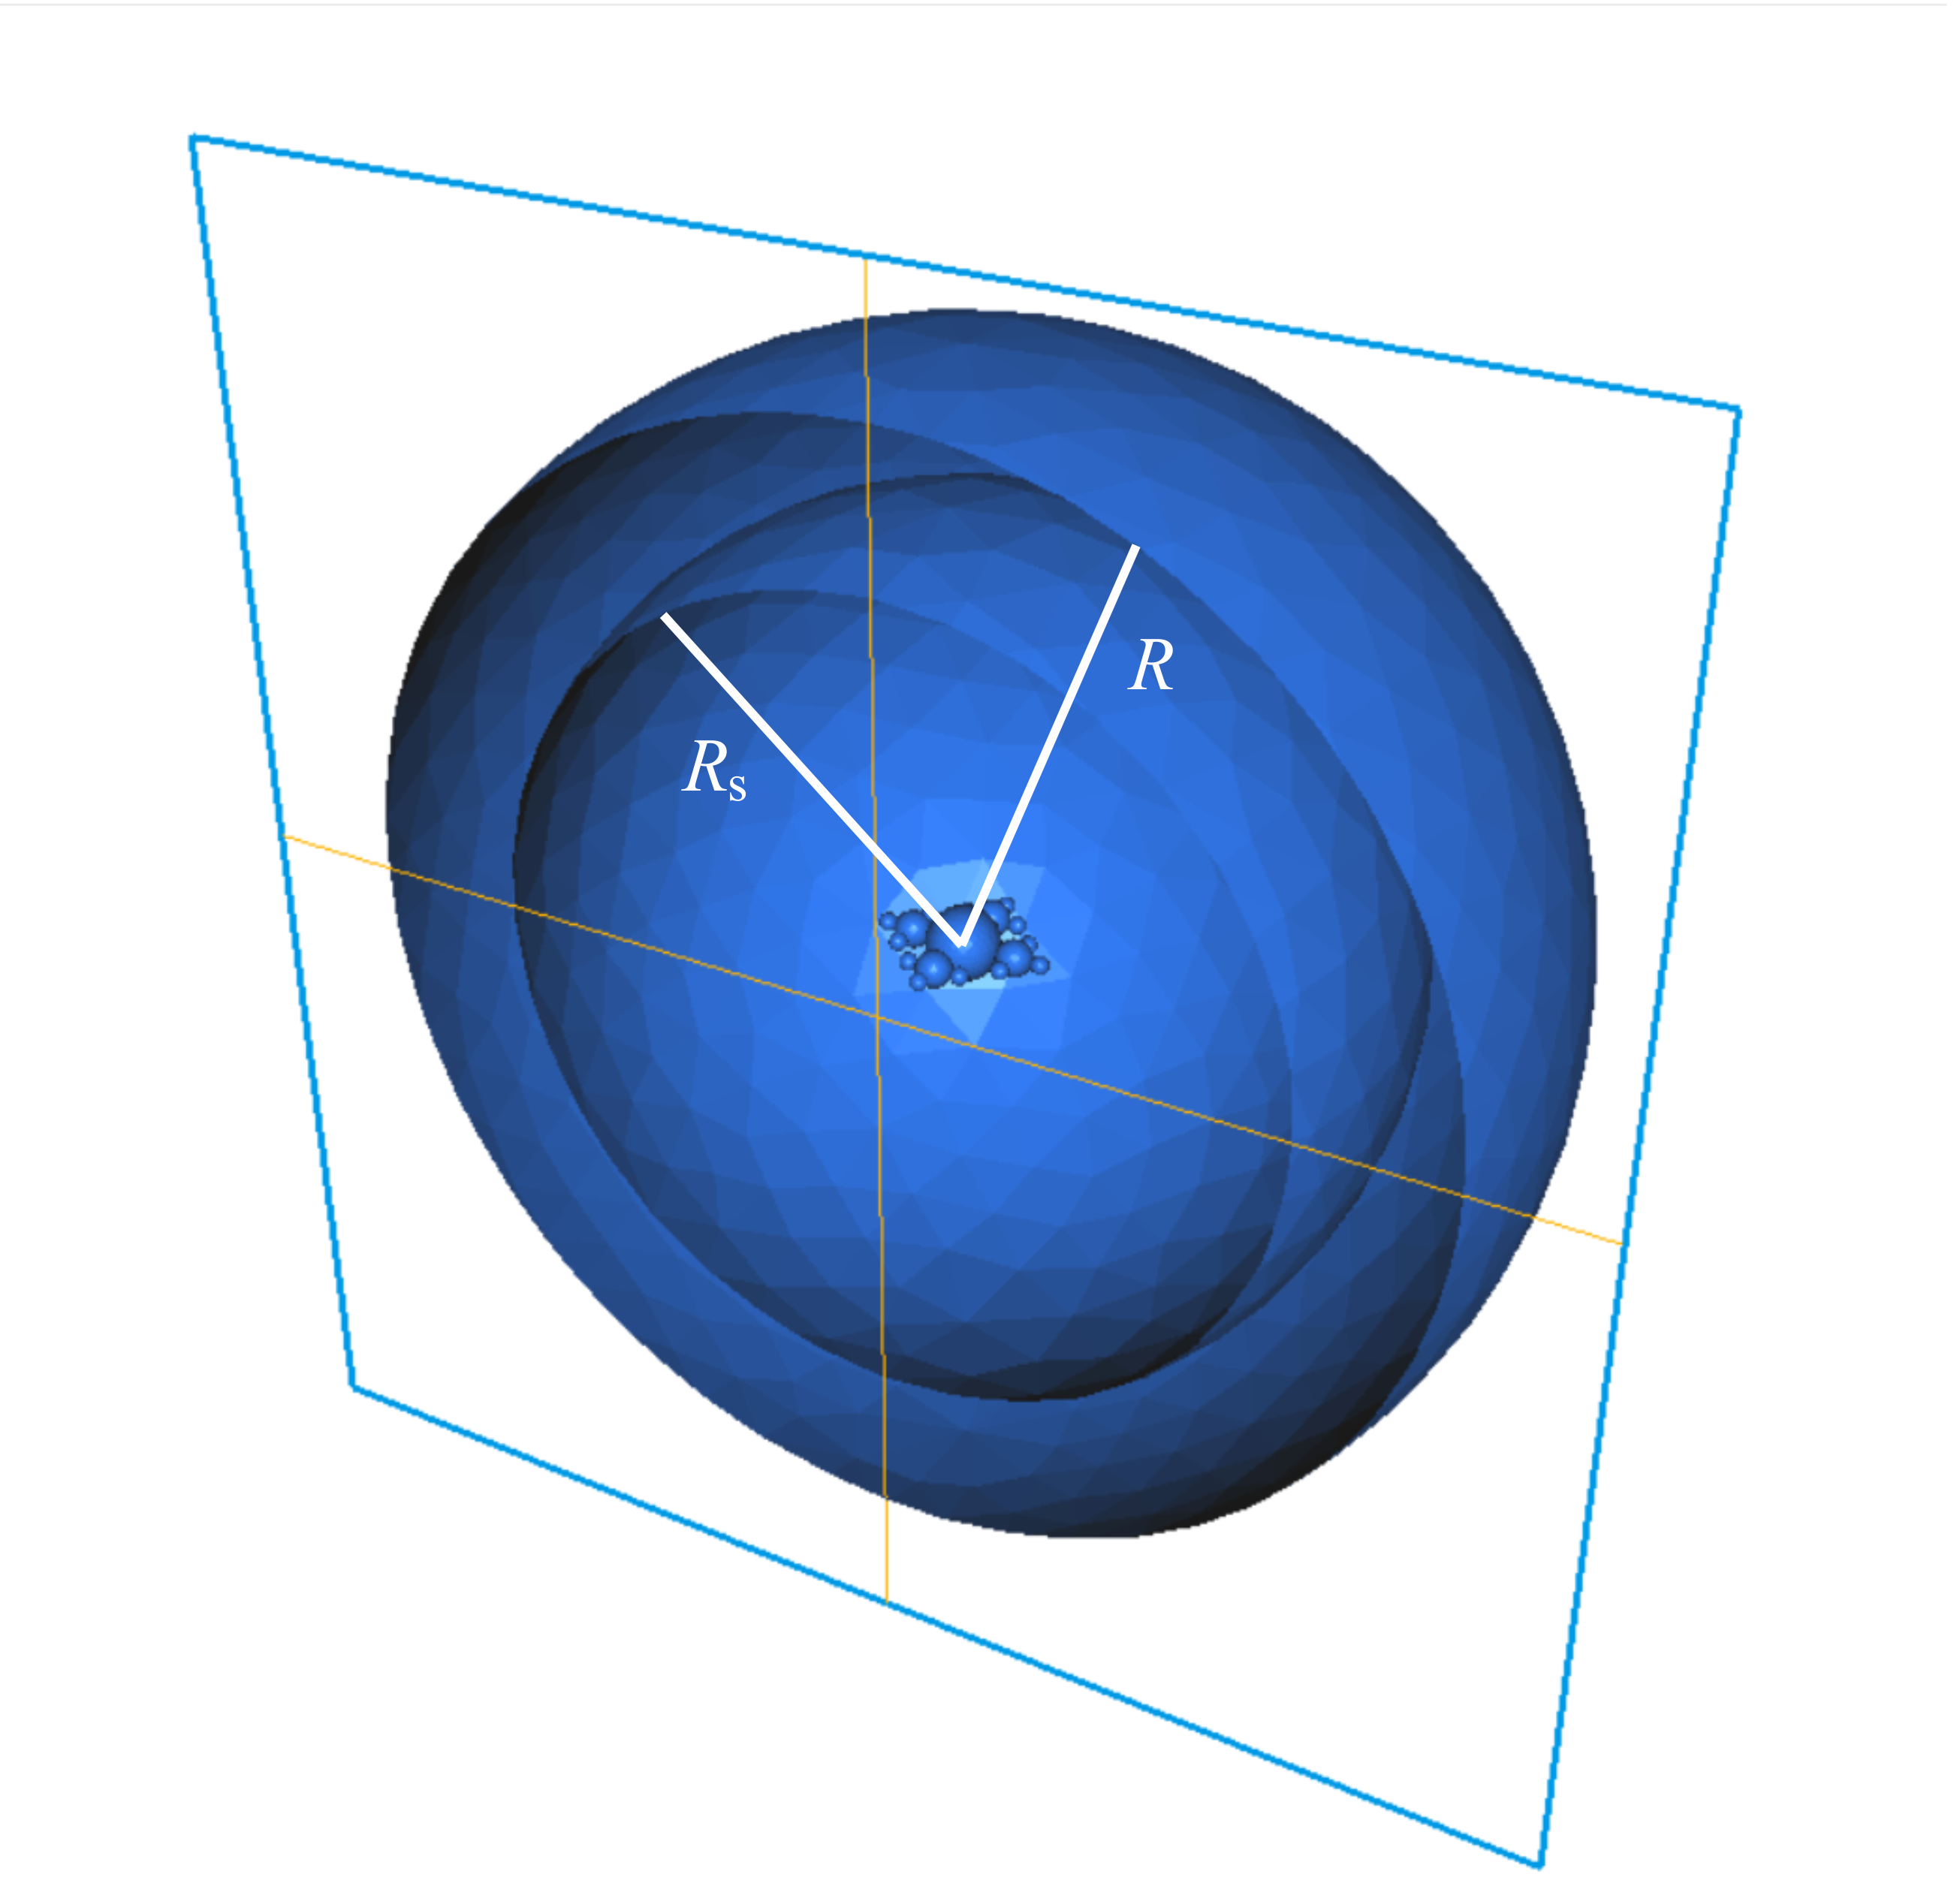
\includegraphics[width=0.6\linewidth]{3td_scattererAndOuterSpheres}
	\caption{}
	\label{fig:3td_scattererAndOuterSpheres}
\end{figure} \\
Теперь нам необходимо записать уравнение, с помощью которого мы и будем производить расчеты полей. Для этого обратимся к Рис.\ref {fig:tes2}
\\
\begin{figure}[h]
	\centering
	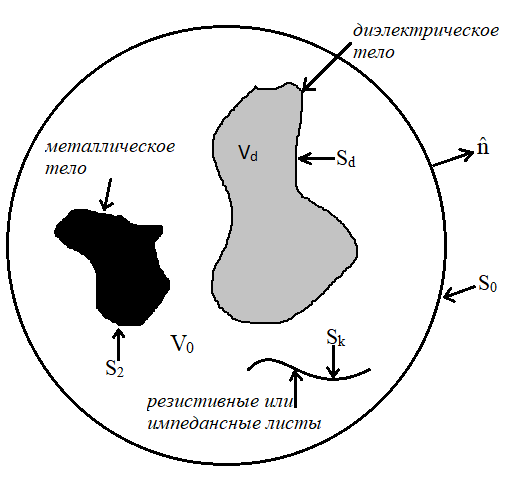
\includegraphics[width=0.6\linewidth]{tes2}
	\caption{}
	\label{fig:tes2}
\end{figure}
\\
Вычислительная область ($ V_{0} $) ограничена поверхностью ($ S_{0} $) и может содержать различные рассеивающие объекты, такие как неоднородные диэлектрики ($ V_{d} $), металлические тела ($ S_{2} $) и резистивные или импедансные листы ($ S_{k} $).\\
Метод конечных элементов позволяет легко моделировать рассеиватели произвольной формы и неоднородные области, не предъявляя жестких требований к их форме, размеру и составу.  \\
Ввиду того, что наш интерес ограничен рассеянием, плотности электрического и магнитного тока будут равны нулю.
С учетом граничных условий на рассеивателе (ях), следует рассмотреть его средневзвешенное значение, дающее так называемую слабую форму векторного волнового уравнения. Для векторной функции $ \vec{\cal{E}} $:\\
\begin{equation}\label{a1}
	\iiint\limits_{V_{0}}^{} \left\{\left[ \nabla \times \left[ \dfrac{1}{\mu_{r}}\nabla \times \vec{E}\right]\right]\cdot \vec{\cal{E}} - k_{0}^{2} \epsilon_{r}\vec{E} \cdot \vec{\cal{E}} \right\}d\upsilon = 0
\end{equation}
Однако уравнение должно выполняться для каждого из малых объемов, а не в каждой точке $ V_{0} $. Из-за двойного завитка, прямое численное решение уравнения (\ref{a1}) требует расширения $ \vec{E} $ с помощью базисных функций $ S_{0} $ более высокого порядка, и мы также можем получить асимметричную систему. Чтобы избежать этих трудностей и облегчить соблюдение граничных условий, традиционный подход состоит в том, чтобы использовать первую векторную идентичность Грина и переписать формулу: \\
\begin{equation}
\iiint\limits_{V_{0}}^{} \left[ \dfrac{1}{\mu_{r}}[\nabla \times \vec{E}] \cdot [\nabla \times \vec{\cal{E}}] - k_{0}^{2} \epsilon_{r}\vec{E} \cdot \vec{\cal{E}} \right]d\upsilon - jk_{0}Z_{0} \oiint [\hat{n} \times \vec{H}] \cdot \vec{\cal{E}}ds = 0,
\end{equation}
где $ \vec{H} $ - полное магнитное поле, удовлетворяющее уравнению Максвелла $ \nabla \times \vec{E} - jk_{0}Z_{0}\vec{H}  $, $ \vec{E} $ - полная напряженность электрического поля, $ \epsilon_{r} $ и $ \mu_{r} $ - обозначают относительную диэлектрическую и магнитную проницаемость, $ k_{0} $ - волновое число в свободном пространстве, $ Z_{0} $ - собственный импеданс свободного пространства. Мы можем решить его численно для $ \vec{E} $, дискретизировав объем $ V_{0} $ и расширив $ \vec{E} $ подходящим, скажем, линейным расширением внутри каждого из подобъемов $V_{e}$. Также необходимо обеспечить соблюдение всех необходимых граничных условий в пределах $V_{0}$ и на $S_{0}$, что подразумевает исключение $\vec{H}$, связав его с $\vec{E}$. \\
Учитывая, что наш интерес заключается в получении рассеяния тела, освещаемого плоской волной, $S_{0}$ служит только в качестве искусственной поверхности для завершения бесконечной вычислительной области. В самом деле, если $S_{0}$ находится далеко от рассеивателя, мы можем тогда вызвать условие излучения Зоммерфельда:
\begin{equation}\label{a2}
	jk_{0}Z_{0}\hat{r} \times \vec{H}^{scat} = jk_{0}\hat{r} \times \hat{r} \times \vec{E}^{scat}
\end{equation}
		связав $ \vec{H} $ и $ \vec{E} $, где $ \hat{r} $ - нормаль к сферической поверхности $ S_{0} $ и
\begin{equation}
	\vec{H}^{scat} = \vec{H} - \vec{H}^{inc},\quad \vec{E}^{scat} = \vec{E} - \vec{E}^{inc}
\end{equation}
Обозначим рассеянные поля, связанные с возбуждением плоской волны ($ \vec{E}^{inc} $, $ \vec{H}^{inc} $).
Очевидно, что требование, чтобы $ S_{0} $ располагалась далеко от рассеивателя, значительно увеличивает вычислительный объем, что приводит к непрактично большим системам при дискретизации уравнения. Это побудило к использованию поглощающих граничных условий более высокого порядка, которые можно наносить на поверхность, находящуюся в ближней зоне рассеивателя, без существенного снижения точности решения.Их целью является устранение обратных отражений от $ S_{0} $. Они обеспечивают приблизительную связь между $\vec{E}$ и $\vec{H}$ на поверхности $ S_{0} $, которую мы получаем, предполагая расширение поля в обратных степенях r, радиальное расстояние от центра $S_{0}$. Если поглощающие граничные условия аннулируют первые (2m + 1) обратные степени r, то их называют поглощающие граничные условия m-го порядка.
Поглощающие граничные условия нулевого порядка являются условием излучения Зоммерфельда, приведенным в формуле (\ref{a2}), а их вектор второго порядка имеет вид:
\begin{equation}\label{a3}
	-jk_{0}Z_{0}\hat{n} \times \vec{H}^{scat} = jk_{0}\vec{E}_{t}^{scat} + \beta \nabla \times [\hat{n}(\nabla \times \vec{E}^{scat})_{n}] + \beta\nabla_{t} (\nabla \cdot \vec{E}_{t}^{scat}).
\end{equation}
В этом уравнении $ \hat{n} $ обозначает внешнюю нормаль к $S_{0}$, $\beta = 1/{2[jk_{0} + (1/r)]}$, а нижние индексы t и n обозначают тангенциальную и нормальную компоненты для $ S_{0} $ соответственно. 
Поглощающие граничные условия (уравнение (\ref{a3})) были получены для сферической поверхности $ S_{0} $, однако, они хорошо работают, когда $ S_{0} $ является кусочно-плоской, чтобы она лучше соответствовала поверхности рассеивателя.
В этом случае $ \beta $ сводится к $ \beta = 1/(2jk_{0}) $.\\
Точно так же мы можем обобщить уравнение (\ref{a2}) для кусочно-плоских поверхностей, положив $ \hat{r} \rightarrow \hat{n} $.\\
Так же отметим, что, поскольку данные поглощающие граничные условия связывают рассеянные поля, лучше всего переписать формулу (\ref{a1}) в терминах рассеянных полей. Делая так, мы получаем:
\begin{align}\label{a4}
	&\iiint\limits_{V_{0}}^{} \left[ \dfrac{1}{\mu_{r}}(\nabla \times \vec{E}^{scat}) \cdot (\nabla \times \vec{\cal{E}}) - k_{0}^{2} \epsilon_{r}\vec{E}^{scat} \cdot \vec{\cal{E}} \right]d\upsilon + 
	\iint\limits_{S_{0}}^{}  P(\vec{E}^{scat}) \cdot \vec{\cal{E}}ds +\notag\\
	&+ 
	\iiint\limits_{V_{d}}^{} \left[ \dfrac{1}{\mu_{r}}(\nabla \times \vec{E}^{inc}) \cdot (\nabla \times \vec{\cal{E}}) - k_{0}^{2} \epsilon_{r}\vec{E}^{inc} \cdot \vec{\cal{E}} \right]d\upsilon +\notag\\
	&+ jk_{0}Z_{0}\iint\limits_{S_{d}}^{} \dfrac{1}{\mu_{r}}(\hat{n} \times \vec{H}^{inc}) \cdot \vec{\cal{E}}ds = 0,
\end{align}
в котором $P(\vec{E^{scat}})$ равно представлению в правой части уравнения (\ref{a2}), $ V_{d} $ - это объем, занимаемый диэлектриками, а $ S_{d} $ - это поверхность между диэлектрическими интерфейсами. Мы вывели последние два интеграла в формуле (\ref{a4}) снова вызвав первое векторное тождество Грина и отметим, что $ \vec{E^{inc}} $ удовлетворяет волновому уравнению вектора свободного пространства. Очевидно, что (\ref{a4}) относится только к неизвестным $ \vec{E^{scat}} $, и мы можем приступить к его решению.
\subsection{Численная схема и точное решение задачи рассеяния на проводящем цилиндре}
Запишем уравнение Гельмгольца:
\begin{equation}
\Delta H_{z} + k^2H_{z} = 0
\end{equation}
Из этого получаем : 
\begin{equation}
{\rm rot}\vec{H} = i k_{0}\vec{H}
\end{equation}
Отсюда выражаем  $\vec{E}$:
\begin{equation}
	\vec{E} = - \dfrac{i}{k_{0}} \rm rot\vec{H} = - \dfrac{i}{k_{0}} \left(\vec{x_{0}}\dfrac{\partial \vec{H_{z}}}{\partial y} - \vec{y_{0}}\dfrac{\partial \vec{H_{z}}}{\partial x}\right)
\end{equation}
А так же для $ E_{x} и E_{y} $ соответственно:
\begin{align}
	&E_{x} = - 
	\dfrac{i}{k_{0}}
	\dfrac{\partial\vec{H_{z}}}{\partial y} \\
	&E_{y} = \dfrac{i}{k_{0}}
	\dfrac{\partial\vec{H_{z}}}{\partial x}
\end{align}
Для условной поверхности S : \\
\begin{equation}
[\vec{n}, \vec{x_{0}}E_{x} + \vec{y_{0}}E_{y}] = 0
\end{equation}
Таким образом получим интеграл:
\begin{equation}
	\int\limits_{V}^{} \Delta H_{z} \cdot wdv = - \int\limits_{V}^{}(\nabla H_{z}, \nabla w)dv +  \int\limits_{V}^{}(\nabla H_{z} \cdot w)dv
\end{equation}
Так как один из интегралов правой части: 
\begin{equation}
	\int\limits_{V}^{}(\nabla H_{z} \cdot w)dv
\end{equation}
Соответственно равен: 
\begin{equation}
	\int\limits_{V}^{}(\nabla H_{z} \cdot w)dv = \oint\limits_{S}^{} \nabla H_{z}  wds \cdot \vec{n} = 0
\end{equation}
То граничные условия в нашей задаче задавать нет необходимости.
Поэтому получим:
\begin{equation}
	\nabla H_{z} = \vec{x}_{0} \dfrac{\partial H_{z}}{\partial x} - \vec{y}_{0}
	\dfrac{\partial H_{z}}{\partial y}
\end{equation}
Cоответственно используя нормали $n_{x}$ и $n_{y}$  запишем искомое уравнение:
\begin{equation}
	\vec{n}\nabla H_{z} = \dfrac{\partial H_{z}}{\partial n} = 
	n_{x}\dfrac{\partial H_{z}}{\partial x} +
	n_{y}\dfrac{\partial H_{z}}{\partial y}
\end{equation}
Теперь решим ту же самую задачу, но уже точным методом. Для этого в начале найдем уравнения, которые нам понадобятся для решений:
\begin{align}
	&\vec{H} = \vec{r_{0}}H_{z}
	 = 1.e^{-ik_{0}x} = e^{-ik_{0}\rho \rm cos\varphi} = 
	\sum\limits_{m=-\infty}^{\infty} J_{m}(k_{0}\rho)e^{-im(\varphi + \dfrac{\pi}{2})} =\notag\\
	&= \sum\limits_{m=-\infty}^{\infty} (-i)^{m}J_{m}(k_{0}\rho)e^{-im\varphi}
\end{align}
Запишем уравнение Гельмгольца и оператор Лапласа в следующем виде:
\begin{center}
	$ 
	\Delta_{\perp}H_{z} + k_{0}H_{z} = 0, \qquad
	\Delta_{\perp} = \dfrac{1}{\rho}
	\dfrac{\partial}{\partial \rho} 
	(\rho \dfrac{\partial}{\partial \rho}) + 
	\dfrac{1}{\rho^{2}}
	\dfrac{\partial^{2}}{\partial \varphi^{2}} 
	$
\end{center}
Получим:
\begin{equation}
	\dfrac{\partial^{2}}{\partial \rho^{2}}H_{z}  +
\dfrac{1}{\rho}\dfrac{\partial}{\partial \rho}H_{z} +
\dfrac{1}{\rho^{2}}\dfrac{\partial^{2}}{\partial \varphi^{2}}H_{z}+
k_{o}^{2}H_{z} = 0
\end{equation}
Представим $ H_{z} $ как некую $ R(\rho) $ и $ \Phi(\varphi) $:\quad
$ H_{z} = R(\rho)\Phi(\varphi) $, \qquad тогда : \\
\begin{equation}
\Phi^{\prime\prime}(\varphi) + m^2\Phi(\varphi) = 0 \quad -> \Phi(\varphi) = e^{-im\varphi}R^{\prime\prime}(\rho) + \dfrac{1}{\rho} R^{\prime} + (k_{0}^{2} - \dfrac{m^{2}}{\rho^{2}})R = 0
\end{equation}
\\
Отсюда получим, что :
\begin{center}
	$$ R(\rho) = A_{1}H_{m}^{(1)}(k_{0}\rho) + A_{2}H_{m}^{(2)}(k_{0}\rho) $$
\end{center}
Однако \quad  $ A_{1} = 0 $, \quad так как
$\quad \lim\limits_{\rho -> \infty}\sqrt{\rho}
(\dfrac{\partial H_{m}^{(2)}}{\partial \varphi \rho} + ik_{0}H_{m}^{(1)} )
$ \\
В таком случае у нас остается: \\
$$
H_{z} = \sum_{m=-\infty}^{\infty}A_{2m}H_{m}^{(2)}(k_{0}\rho)e^{-im\varphi}
$$
\\
Граничные условия:
\begin{equation}
	E_{\varphi}|_{\rho=a} = 0
\end{equation}
Тогда:
\begin{eqnarray}
&&\vec{E}^{(s)} = - \dfrac{i}{k_{0}\varepsilon} \rm rot\vec{H}^{(s)} = - \dfrac{i}{k_{0}} \dfrac{1}{\rho}
\begin{vmatrix}
\vec{\rho}_{0}& \;\rho \vec{\varphi}_{0}& \; \vec{z}_{0} \\
\dfrac{\partial }{\partial \rho}& \; 
\dfrac{\partial }{\partial \varphi}&\; 
\dfrac{\partial }{\partial z} \\
H_{\rho}&\; \rho H_{\varphi}&\; H_{z}^{(s)}
\end{vmatrix}
= \dfrac{i}{k_{0}} \dfrac{1}{\rho}\left(\vec{\rho}_{0}
\dfrac{\partial H_{z}}{\partial \rho} - \rho\vec{\varphi}_{0}
\dfrac{\partial H_{z}^{(s)}}{\partial \rho}\right)
\\
&&E_{\varphi}^{(s)} = \dfrac{i}{k_{0}}
\dfrac{\partial }{\partial \rho} \sum_{m=-\infty}^{\infty} A_{2m}H_{m}^{(2)}(k_{0}\rho)e^{-im\varphi} =
\dfrac{i}{k_{0}} \sum_{m=-\infty}^{\infty}A_{2m} 
\dfrac{\partial }{\partial \rho}
(H_{m}^{(2)}(k_{0}\rho))e^{-im\varphi}
=
\end{eqnarray}
\begin{equation}
i\sum_{m=-\infty}^{\infty}A_{2m}{H_{m}^{(2)}}^{\prime}(k_{0}\rho)e^{-im\varphi}
\end{equation}
Исходя из граничных условий для падающей и отраженной волны:
\begin{equation}
E_{\varphi}|_{\rho=a} = (E_{\varphi}^{(i)} + E_{\varphi}^{(s)})|_{\rho=a} = \sum_{m=-\infty}^{\infty}
((-i)^{m}J_{m}^{\prime}(k_{0}\rho) + A_{2m}{H_{m}^{(2)}}^{\prime}(k_{0}\rho))e^{-im\varphi}|_{\rho=a} = 0
\end{equation}
Получим искомое выражение:
\begin{align}
&(-i)^{m}J_{m}^{\prime}(k_{0}a) + A_{2m}{H_{m}^{(2)}}^{\prime}(k_{0}a) = 0\\
&A_{2m} = (-i)^{m} \dfrac{J_{m}^{\prime}(k_{0}a)}
{{H_{m}^{(2)}}^{\prime}(k_{0}a)}
\end{align}
\section{Тестирование численной схемы}

Приступим к созданию трехмерной модели в программе FreeFem++ на основе полученных нами выше выражений \cite{bfreefem}.  Для этого выберем наиболее подходящий программный способ реализации 3D объектов, а так же сразу определим, что наш объект будет в виде сферы(у которой тут же зададим радиус и другие параметры). Возьмем сферическую область, в которой будут рассеиваться волны и заключим в нее наш объект - сферу более маленького радиуса заполненного диэлектриком.
Определим параметры характеризующие наше поле,а именно:
	$ \lambda = 10^{-6} $ - длина волны в вакууме в метрах,
	$ c = 299792458 $ - скорость света в вакууме, $ \mu = 4\pi 10^{-7} $ - магнитная проницаемость в свободном пространстве, $ \varepsilon = \dfrac{\mu}{c^{2}} $ - диэлектрическая проницаемость в свободном пространстве, $ Z = \sqrt{\dfrac{\mu}{\varepsilon}} $ - импеданс свободного пространства, $ n = 2 $ - показатель преломления сферы

Радиус внутренней сферы (нашего объекта) зададим в 10 раз меньше длины волны принимаемой для расчетов ($ \lambda = 1 $), а радиус внешней сферы в 4 раза больше. Таким образом получим систему состоящую из двух сфер разного радиуса (одна внутри другой), взаимодействие между которыми опиcываются с помощью уравнений полученных ранее. Однако, прежде чем мы это сделаем, определим в программе область расчетов через радиус внутренней сферы, для случаев когда он больше или меньше радиуса применяемого для вычислений полей в ближней и дальней зоне. Необходимость этого заключается в том, что уравнение должно выполняться для каждого из малых объемов, а не в каждой точке, как было сказано ранее.
\\
Опрелелим k для случаев:
\begin{equation}
	k = 
	\begin{cases}
		1, & r > a\\
		n, & r < a ,\qquad \text{где }a \text{ --- радиус малой сферы}
	\end{cases}
\end{equation}
Далее добавим цикл, который ввиду гармонической зависимости от времени будет производить перерасчет данных и выводить результаты на экран, благодаря чему получится наглядная анимированная картина поля. А так же добавим возможность сохранения полученных данных для Matlab. После того, как мы посчитали дифракцию на сфере, перейдем непосредственно к расчету сечения рассеяния и сечения поглощения. Если на рассеивающий элемент падает волна с интенсивностью I(под интенсивностью понимается поток энергии через единичную площадку), то полная рассеянная мощность S будет пропорциональна I. Коэффициент пропорциональности между этими величинами $ \sigma_s $ называется полным сечением рассеяния и имеет размерность площади:
\begin{equation}
	\sigma_s = \dfrac{S}{I} 
\end{equation}
Так же введем понятие дифференциального сечения рассеяния
 $ \sigma_d(\theta,\varphi) $. Пусть $ dS(\theta, \varphi) $ - полная мощность, рассеянная в пределах телесного угла d$ \Omega $ в направлении $ (\theta,\varphi) $, тогда:
 \begin{center}
 	$ \sigma_d(\theta,\varphi) = \lim\limits_{d\Omega\rightarrow\infty} \dfrac{dS(\theta, \varphi)}{Id\Omega}. $s
 \end{center}
Приминительно к нашей задаче, это выражение примет вид:
\begin{equation}
\sigma_d(\theta,\varphi) = \lim\limits_{R\rightarrow\infty} \dfrac{R^2 S_r(\theta, \varphi)}{S_i}.
\end{equation}
Здесь вектор Пойнтинга падающей волны
\begin{equation}
{\vec S}_i = \dfrac{c}{8\pi} \left[{\vec E}_i \times {\vec H}^*_i\right],
\end{equation}
радиальная компонента вектора Пойнтинга рассеянных волн
\begin{equation}
{S}_r = \dfrac{c}{8\pi} \left[{\vec E}_s \times {\vec H}^*_s\right] \cdot {\vec \rho}_0
\end{equation}
В нашем случае при расчётах необходимо будет взять значения вектора Пойнтинга рассеянных волн на поверхности с фиксированным значением $R$ (приемлемо, если $R=3\lambda$, т.к. внешняя граница удалена на расстояние $4\lambda$).\\
Наиболее простой способ расчёта $S_r$ через компоненты в декартовой системе координат:
\begin{equation}
{S}_r = S_x \rm cos(\varphi)\sin(\theta) + S_y \sin(\varphi)\sin(\theta) + S_z \rm cos(\theta).
\end{equation}
Здесь
\begin{eqnarray}
& S_x = \dfrac{c}{8\pi} \left(E_y H_z^* - E_z H_y^*\right),\nonumber\\
& S_y = \dfrac{c}{8\pi} \left(E_z H_x^* - E_x H_z^*\right),\nonumber\\ & S_z = \dfrac{c}{8\pi} \left(E_x H_y^* - E_y H_x^*\right).
\end{eqnarray}
Предполагается, что поля относятся к рассеянному полю (индеркс $s$ опущен).
Компоненты магнитного поля находим из уравнения Максвелла
\begin{equation}
{\vec H} = \dfrac{i}{k_0} {\rm \rm rot} \vec{E}.
\end{equation}
Полное сечение рассеяния находится как интеграл по полному телесному углу:
\begin{equation}
\sigma_s = \int_{4\pi} \sigma_d d\Omega.
\end{equation}
Сечение поглощения определяется как отношение полной мощности, теряемой первичной волной и преобразующейся в тепло в данной локальной области, к плотности потока энергии(интенсивности) в первичной волне, его находим как:
\begin{equation}
\sigma_a = \left(\int_V \dfrac{1}{2}\omega\varepsilon''|{\vec E}|^2 d V\right)/S_i.
\end{equation}
В случае, если падающее поле имеет единичную амплитуду ($|E_i|=1$):
\begin{equation}
\sigma_a = \int_V k \varepsilon''|{\vec E}|^2 d V.
\end{equation}
Здесь интегрирование проводится по области занятой диэлектрическим рассеивателем.\\
Вычисление действительной и мнимой частей диэлектрической проницаемости на основе коэффициента преломления будет выглядеть как:
\begin{equation}
\varepsilon' - i \varepsilon'' = (n'-i n'')^2.
\end{equation}
Отсюда действительная $ \varepsilon' $ и мнимая $ \varepsilon'' $ часть будут соответственно равны:
\begin{equation}
\varepsilon' = (n')^2 - (n'')^2,\quad \varepsilon'' = 2 n'n''.
\end{equation}

\section{Результаты численных расчётов}
Однако перед этим, найдем рассеяние на цилиндре численным и точным методом решения, чтобы убедиться в правильности получаемых данных.
\begin{figure}[h!]
	\centering
	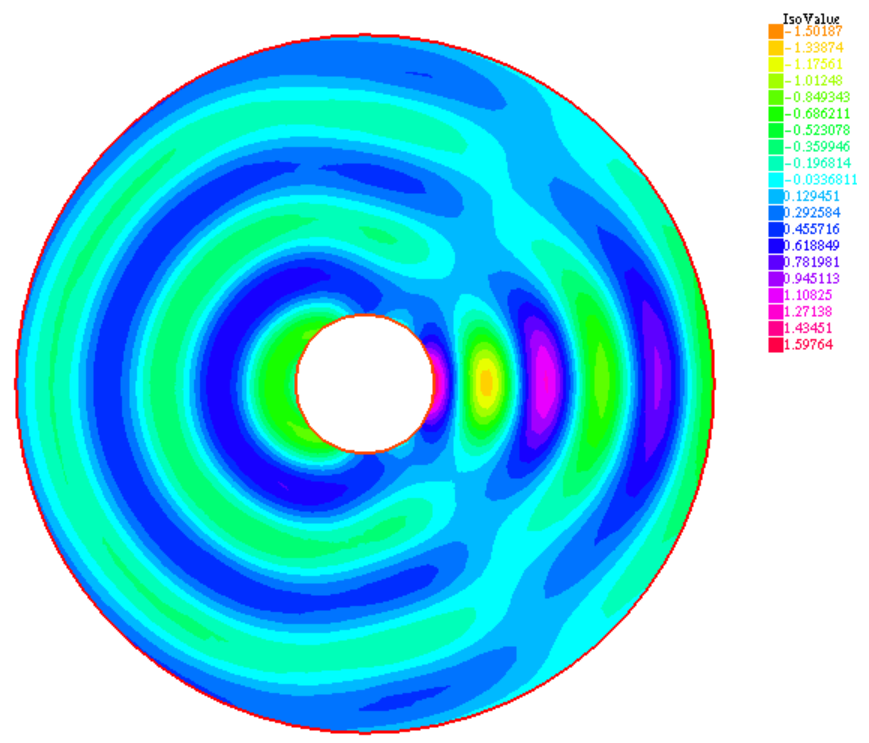
\includegraphics[width=0.8\linewidth]{sc1.png}
	\caption{Численный метод}
	\label{fig:sc1}
\end{figure} 
\newpage
\begin{figure}[h!]
	\centering
	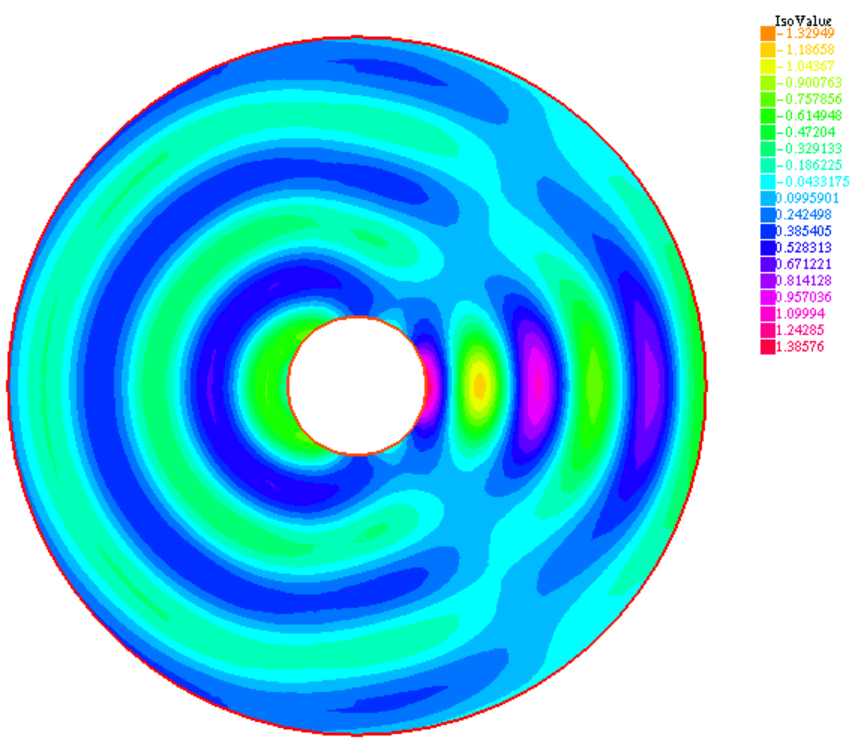
\includegraphics[width=0.8\linewidth]{sc2.png}
	\caption{Точный метод}
	\label{fig:sc2}
\end{figure}
Как видно из Рис. \ref{fig:sc1} и \ref{fig:sc2} при рассеянии плоской волны на цилиндре мы получили практически одинаковые значения поля в точках с точностью до фазы, не смотря на то, что вычисление производилось разными математическими методами, что в свою очередь показывает правильную постановку задачи и ее верное решение. \\ 
Ниже приведены результаты численных расчётов сечения рассеяния и сечения поглощения для рассеивателей, состоящих из одного шара, пяти и семнадцати. Шары заполнены золотом \cite{Olmon2012}, серебром \cite{Yang2015}, либо медью \cite{Querry1985}. Для расчетов применяются оптические плотности материалов.\\
С ростом частоты, происходит существенное уменьшению диапазона длин волн как для сечения поглощения (например \ref{fig:singleCopperSphereAbsorptionSection},  \ref{fig:singleSilverSphereAbsorptionSection}, \ref{fig:singleGoldSphereAbsorptionSection}), так и сечения рассеяния (например \ref{fig:singleCopperSphereAbsorptionSection}, \ref{fig:singleSilverSphereAbsorptionSection}, \ref{fig:singleGoldSphereAbsorptionSection}), для которого зависимость будет ближе к гиперболической. В частности графики (Рис. \ref{fig:singleCopperSphereCrossSection}, \ref{fig:singleSilverSphereCrossSection}, \ref{fig:singleGoldSphereCrossSection}) будут напоминать график гиперболического косеканса (Рис. \ref{fig:csch}), причем в дальнейшем при увеличении числа рассеивателей эта зависимость будет сохраняться, в случае с 5 сферами (Рис. \ref{fig:fiveCopperSphereCrossSection}, \ref{fig:fiveSilverSphereCrossSection}, \ref{fig:fiveGoldSphereCrossSection}) или 17 сферами (Рис. \ref{fig:seventeenCopperSphereCrossSection}, \ref{fig:seventeenSilverSphereCrossSection}, \ref{fig:seventeenGoldSphereCrossSection}). Получается, что для рассеяния волны требуется высокая частота, но лишь в ограниченном диапазоне длин волн, так как добиться отрицательного коэффициента преломления, можно лишь когда диэлектрическая проницаемость и магнитная восприимчивость так же будут отрицательными, однако верно это будет в небольшом диапазоне длин волн, что подтверждается теорией фрактальных антенн и метаматериалов представленной ранее. И если со вторым все более-менее понятно, то как можно объяснить требования высокой частоты? Чтобы добиться отрицательной реакции, необходимо подбирать частоты колебаний при использовании резонансной характеристики среды таким образом, что бы силы, создаваемые электрическими и магнитными полями воздействовали в противоположном направлении движению электронов. Так, если толкнуть качели, то они начнут двигаться с частотой собственных колебаний и подталкивая их с этой частотой мы будем входить в резонанс, тем самым увеличивать амплитуду. Если же мы начнем толкать их с более высокой частотой, то в какой-то момент наши толчки перестанут совпадать с колебаниями по фазе и рука ударится о движущиеся ей навстречу качели. Похожим образом ведут себя электроны, входящие в противофазу и начинающие сопротивляться "толчкам" электромагнитного поля.
\begin{figure}[h!]
	\centering
	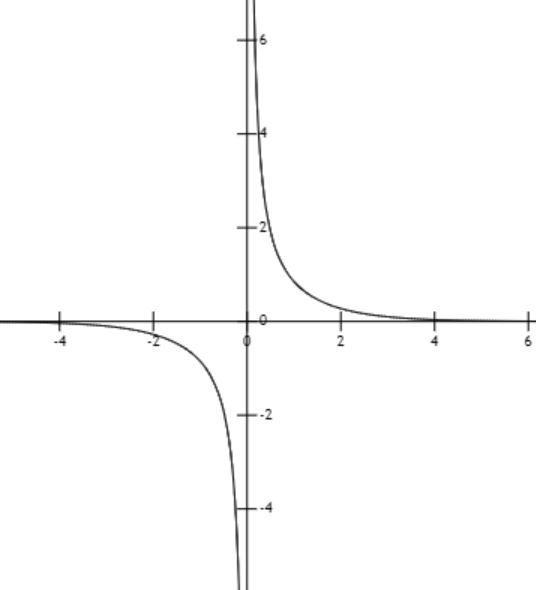
\includegraphics[width=0.32\linewidth]{csch}
	\caption{y = csch (Гиперболический косеканс)}
	\label{fig:csch}
\end{figure}\\
Увеличение элементов рассеивателя приводит расширению диапазона длин волн для сечения поглощения с одиночной сферой (Рис.\ref{fig:singleCopperSphereAbsorptionSection},\ref{fig:singleGoldSphereAbsorptionSection}),5 сферами (Рис.\ref{fig:fiveCopperSphereAbsorptionSection},\ref{fig:fiveGoldSphereAbsorptionSection}), и 17 сферами (Рис.\ref{fig:seventeenCopperSphereAbsorptionSection},\ref{fig:seventeenGoldSphereAbsorptionSection}) в случае если материал – медь и в меньшей степени если это золото, однако с каждой новой итерацией изменение менее значительно. Тоже самое нам говорит теория фрактальных антенн, увтерждающая, что весомый вклад вносят лишь пара первых итераций, которые называют кривыми, заполняющие пространство (Space Filling Curve) \cite{b12}\cite{b13}, а дальнейшее увеличение элементов не даст столь значительного эффекта.  В случае с серебром (Рис.\ref{fig:singleSilverSphereAbsorptionSection},\ref{fig:fiveSilverSphereAbsorptionSection},\ref{fig:seventeenSilverSphereAbsorptionSection}), это изменение очень мало и заметно лишь через одну итерацию. Для сечения рассеяния увеличение числа элементов существенных изменений не вносит. Так же стоит помнить, что уменьшая размер антенны (каждая новая итерация сфер меньше предыдущей в 2 раза), мы уменьшаем длину волны, для которой среда будет иметь отрицательный показатель преломления. \\
Изменение материала рассеивателя приводит к изменению максимальной частоты и расширению/сужению диапазона длин волн в зависимости от того, какой материал был выбран. Так же исходя из теории стоит помнить, что чем больше мощности первичной волны будет поглощено в сечении поглощении материала, тем больше его будет преобразовано в тепло. Конечно, речь не идет о каких-то больших значениях, однако этот факт тоже стоит иметь ввиду.
Из графиков (Рис. \ref{fig:singleCopperSphereAbsorptionSection} и \ref{fig:singleSilverSphereAbsorptionSection}, \ref{fig:fiveCopperSphereAbsorptionSection} и \ref{fig:fiveSilverSphereAbsorptionSection}, \ref{fig:seventeenCopperSphereAbsorptionSection} и \ref{fig:seventeenSilverSphereAbsorptionSection}) видно, что большее поглощение происходит на медной сфере, а меньшее на серебряной. Золотая сфера в это случае занимает промежуточную позицию. В случае с сечением рассеяния (Рис. \ref{fig:singleCopperSphereCrossSection} и \ref{fig:singleGoldSphereCrossSection}, \ref{fig:fiveCopperSphereCrossSection} и \ref{fig:fiveGoldSphereCrossSection}, \ref{fig:seventeenCopperSphereCrossSection} и \ref{fig:seventeenGoldSphereCrossSection}) медь и золото демонстрируют почти одинаковые результаты, однако у первого материала максимальная частота не много выше, серебро же (Рис. \ref{fig:singleSilverSphereCrossSection}, \ref{fig:fiveSilverSphereCrossSection}, \ref{fig:seventeenSilverSphereCrossSection}) показывает гораздо меньшие результаты. \\
Из всего вышеперечисленного, можно сделать вывод, что для работы на более высоких частотах необходимо использовать более короткие длины волн определенного диапазона, а так же подбирать частоту колебаний при использовании резонансной характеристики среды. Для работы же на более длинных волнах требуется увеличить количество элементов рассеивателя или изменить материал, из которого они состоят.

\begin{figure}[h!]
	\centering
	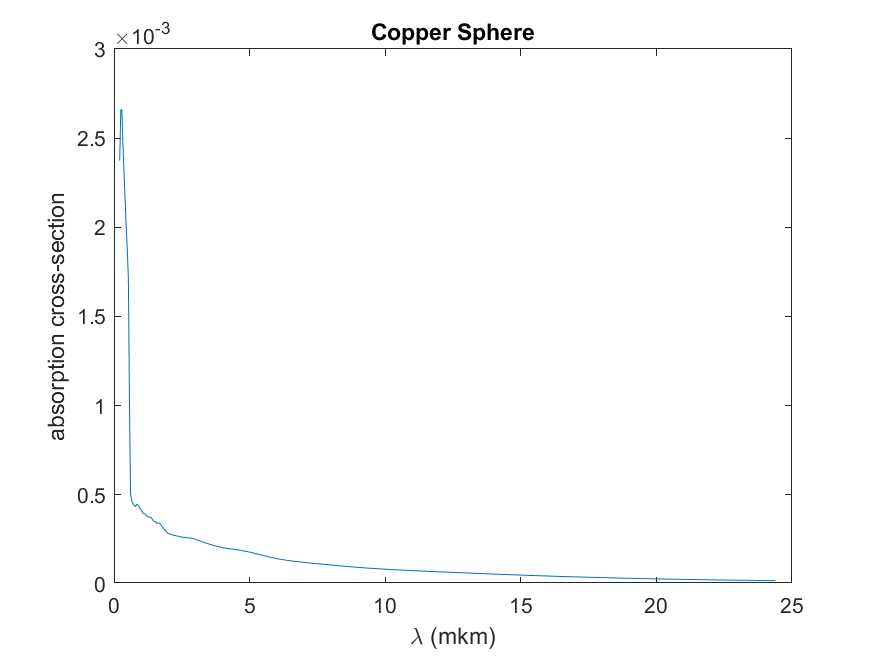
\includegraphics[width=0.5\linewidth]{singleCopperSphereAbsorptionSection}
	\caption{Поглощение на одиночной медной сфере}
	\label{fig:singleCopperSphereAbsorptionSection}
\end{figure}
\begin{figure}[h!]
	\centering
	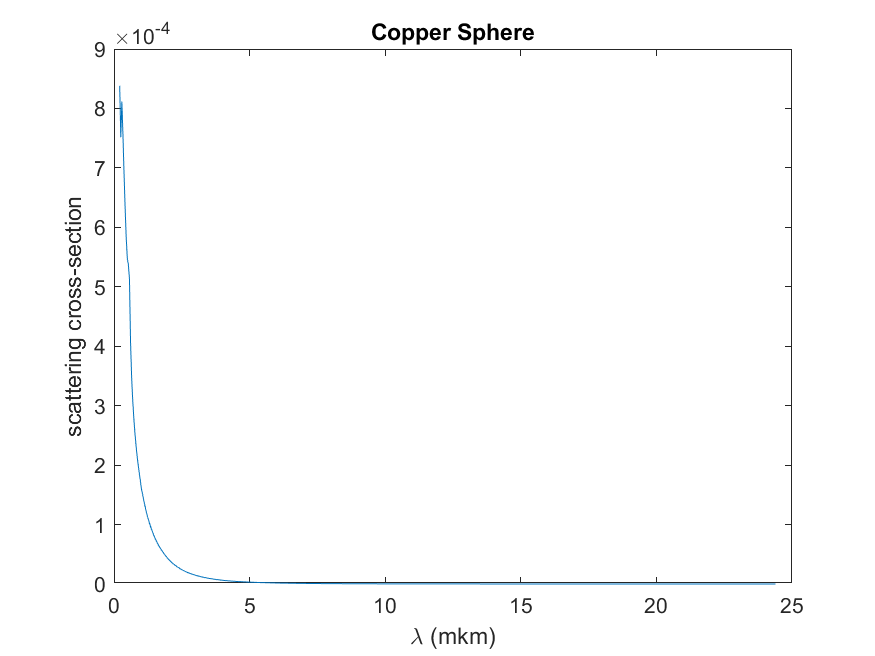
\includegraphics[width=0.5\linewidth]{singleCopperSphereCrossSection}
	\caption{Рассеяние на одиночной медной сфере}
	\label{fig:singleCopperSphereCrossSection}
\end{figure}
\begin{figure}[h!]
	\centering
	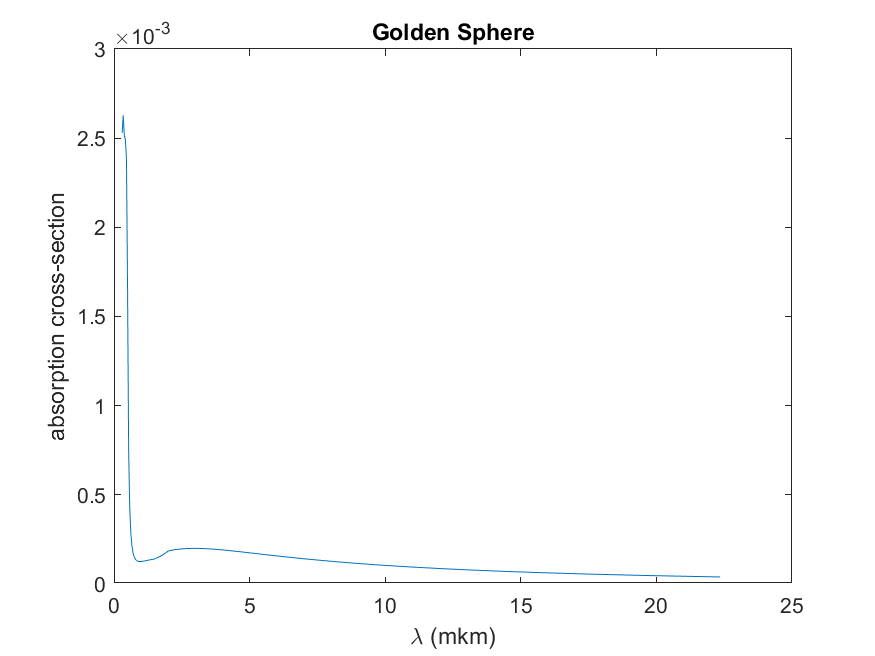
\includegraphics[width=0.5\linewidth]{singleGoldSphereAbsorptionSection}
	\caption{Поглощение на одиночной золотой сфере}
	\label{fig:singleGoldSphereAbsorptionSection}
\end{figure}
\begin{figure}[h!]
	\centering
	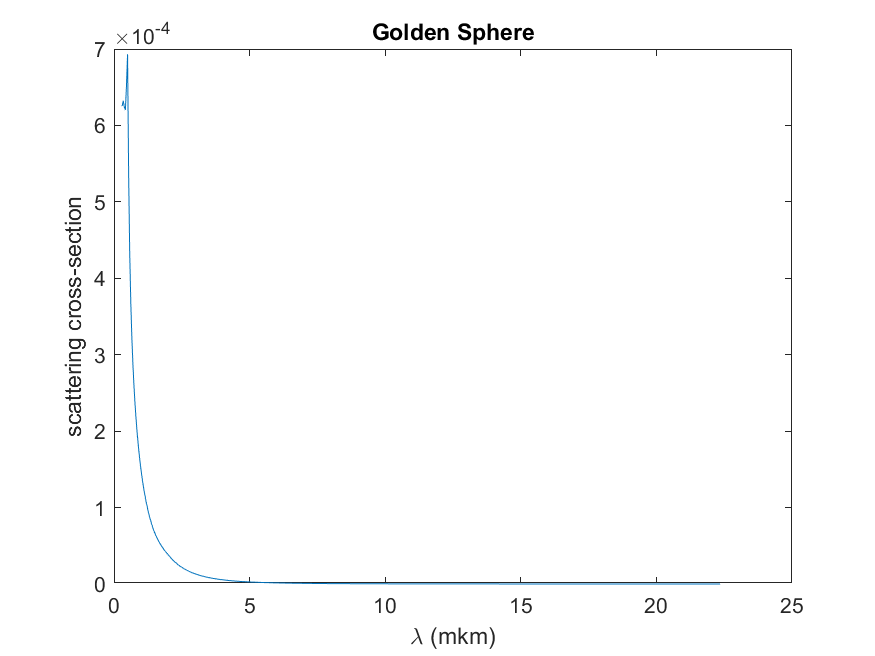
\includegraphics[width=0.5\linewidth]{singleGoldSphereCrossSection}
	\caption{Рассеяние на одиночной золотой сфере}
	\label{fig:singleGoldSphereCrossSection}
\end{figure}
\begin{figure}[h!]
	\centering
	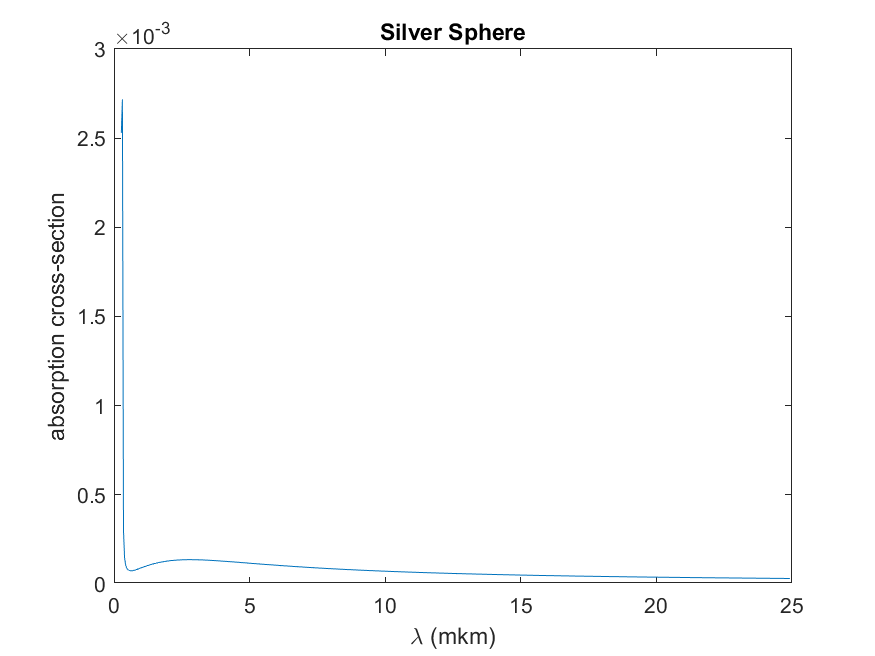
\includegraphics[width=0.5\linewidth]{singleSilverSphereAbsorptionSection}
	\caption{Поглощение на одиночной серебряной сфере}
	\label{fig:singleSilverSphereAbsorptionSection}
\end{figure}
\begin{figure}[h!]
	\centering
	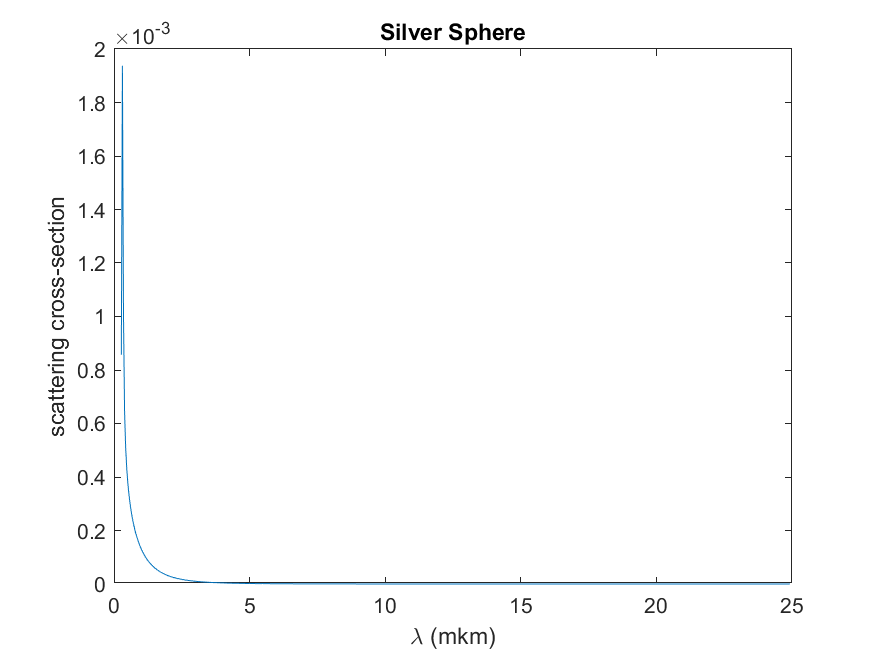
\includegraphics[width=0.5\linewidth]{singleSilverSphereCrossSection}
	\caption{Рассеяние на одиночной серебряной сфере}
	\label{fig:singleSilverSphereCrossSection}
\end{figure}
\begin{figure}[h!]
	\centering
	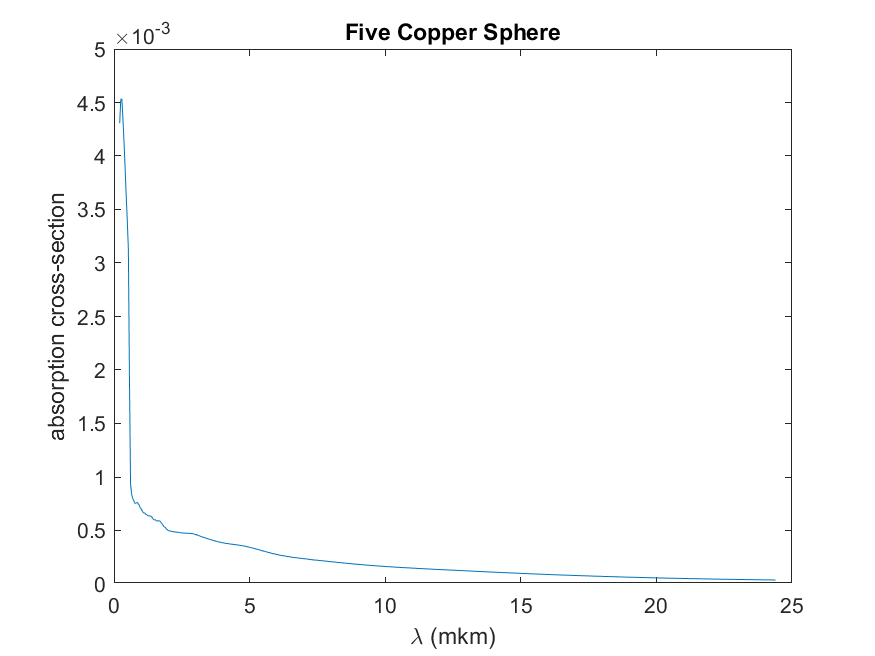
\includegraphics[width=0.5\linewidth]{fiveCopperSphereAbsorptionSection}
	\caption{Поглощение на 5 медных сферах}
	\label{fig:fiveCopperSphereAbsorptionSection}
\end{figure}
\begin{figure}[h!]
	\centering
	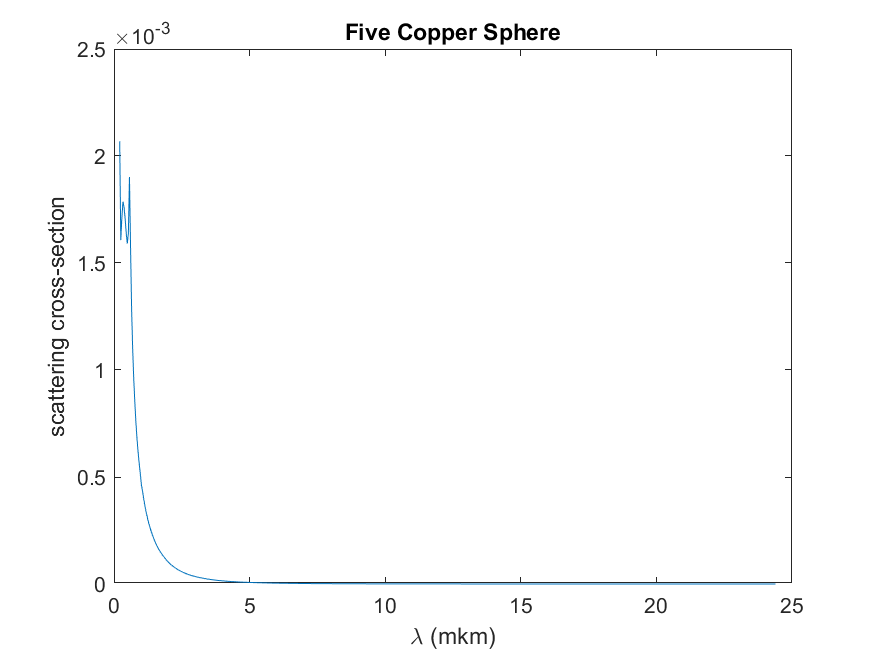
\includegraphics[width=0.5\linewidth]{fiveCopperSphereCrossSection}
	\caption{Рассеяние на 5 медных сферах}
	\label{fig:fiveCopperSphereCrossSection}
\end{figure} 
\begin{figure}[h!]
	\centering
	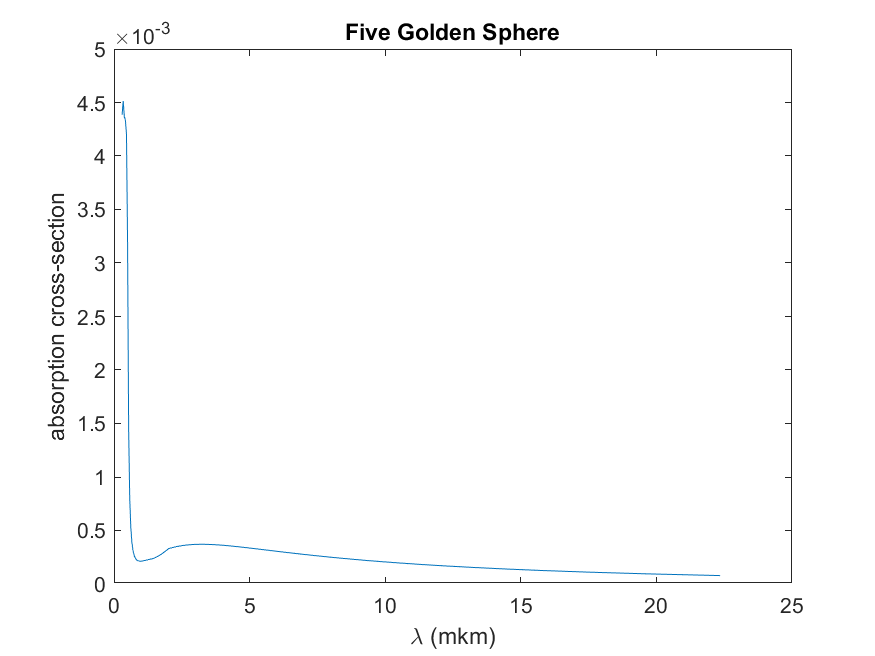
\includegraphics[width=0.5\linewidth]{fiveGoldSphereAbsorptionSection}
	\caption{Поглощение на 5 золотых сферах}
	\label{fig:fiveGoldSphereAbsorptionSection}
\end{figure}
\begin{figure}[h!]
	\centering
	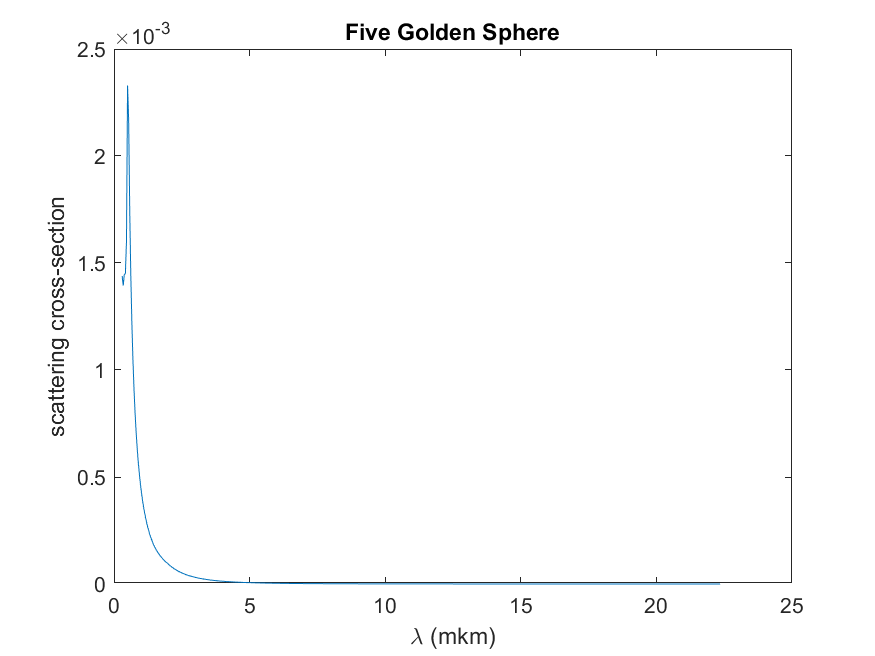
\includegraphics[width=0.5\linewidth]{fiveGoldSphereCrossSection}
	\caption{Рассеяние на 5 золотых сферах}
	\label{fig:fiveGoldSphereCrossSection}
\end{figure}
\begin{figure}[h!]
	\centering
	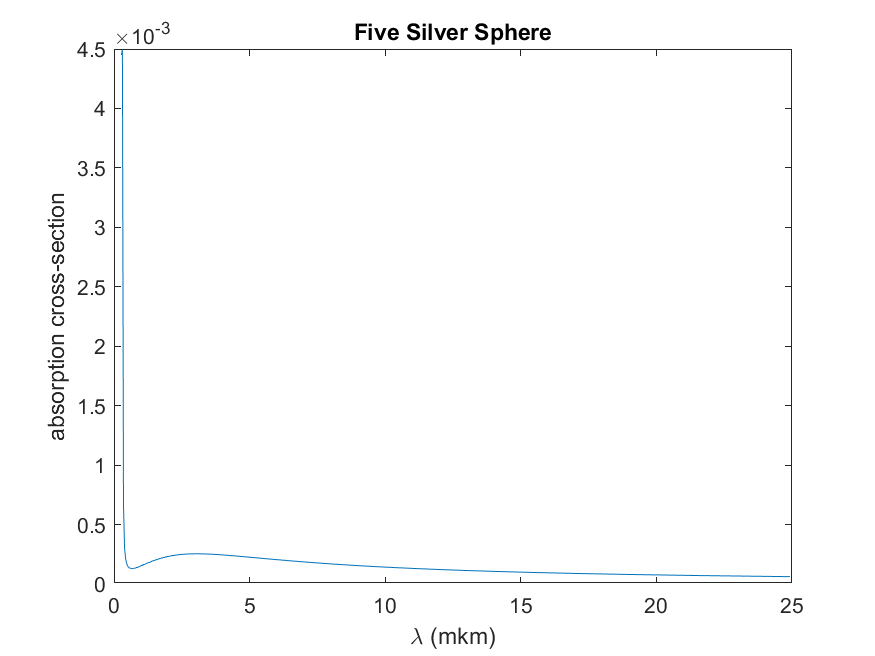
\includegraphics[width=0.5\linewidth]{fiveSilverSphereAbsorptionSection}
	\caption{Поглощение на 5 серебряных сферах}
	\label{fig:fiveSilverSphereAbsorptionSection}
\end{figure} 
\begin{figure}[h!]
	\centering
	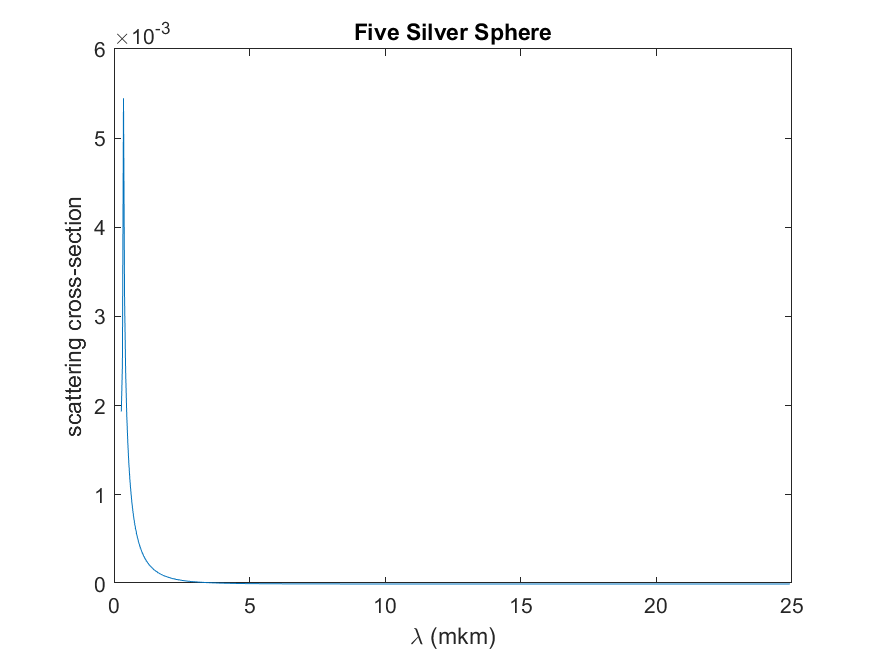
\includegraphics[width=0.5\linewidth]{fiveSilverSphereCrossSection}
	\caption{Рассеяние на 5 серебряных сферах}
	\label{fig:fiveSilverSphereCrossSection}
\end{figure} 
\begin{figure}[h!]
	\centering
	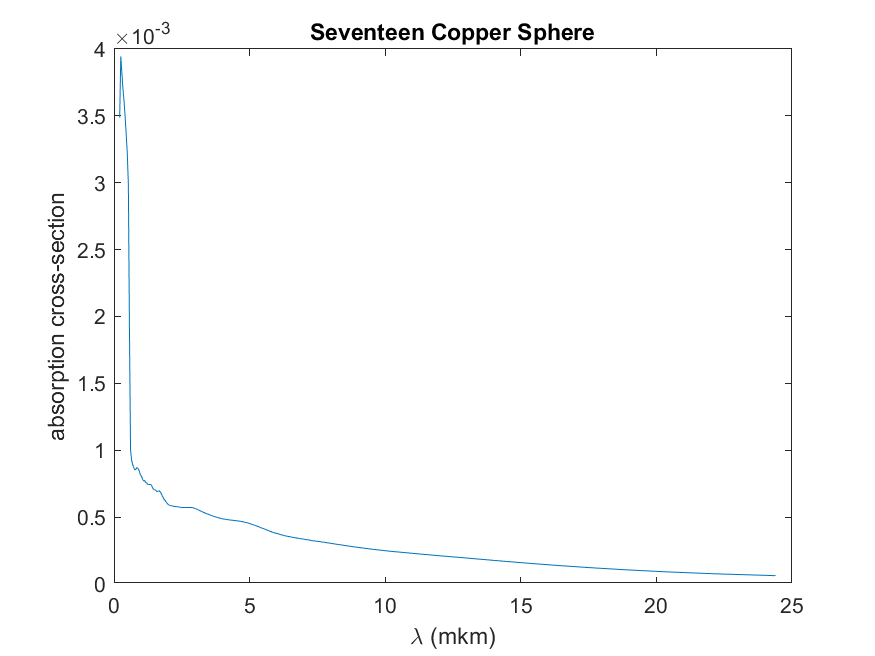
\includegraphics[width=0.5\linewidth]{seventeenCopperSphereAbsorptionSection}
	\caption{Поглощение на 17 медных сферах}
	\label{fig:seventeenCopperSphereAbsorptionSection}
\end{figure} 
\begin{figure}[h!]
	\centering
	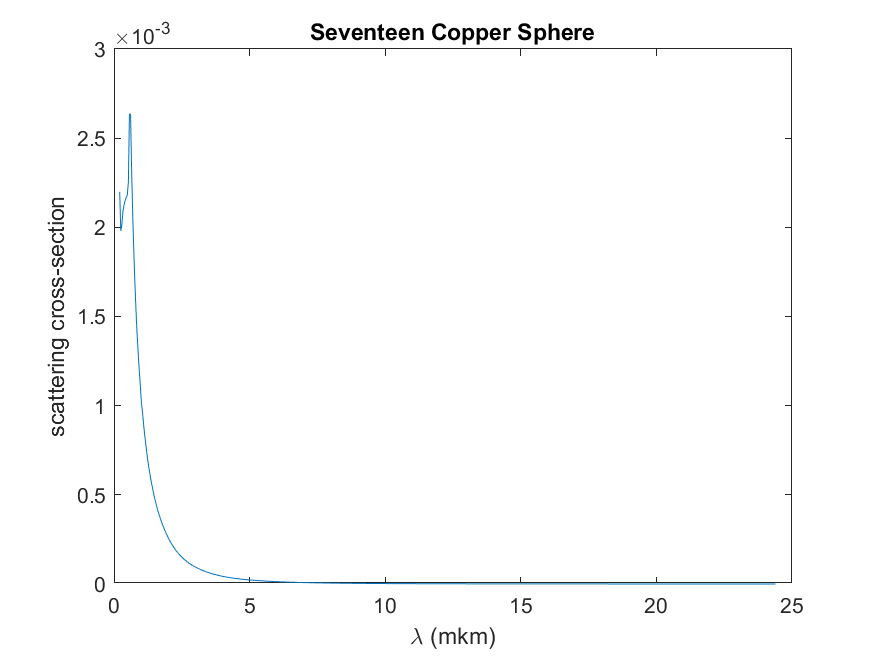
\includegraphics[width=0.5\linewidth]{seventeenCopperSphereCrossSection}
	\caption{Рассеяние на 17 медных сферах}
	\label{fig:seventeenCopperSphereCrossSection}
\end{figure}
\begin{figure}[h!]
	\centering
	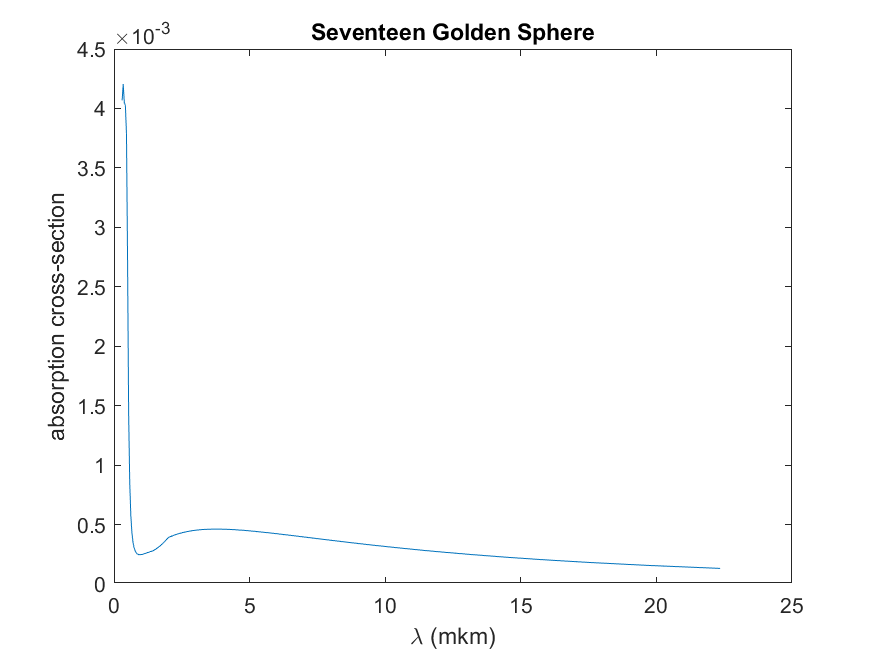
\includegraphics[width=0.5\linewidth]{seventeenGoldSphereAbsorptionSection}
	\caption{Поглощение на 17 золотых сферах}
	\label{fig:seventeenGoldSphereAbsorptionSection}
\end{figure} 
\begin{figure}[h!]
	\centering
	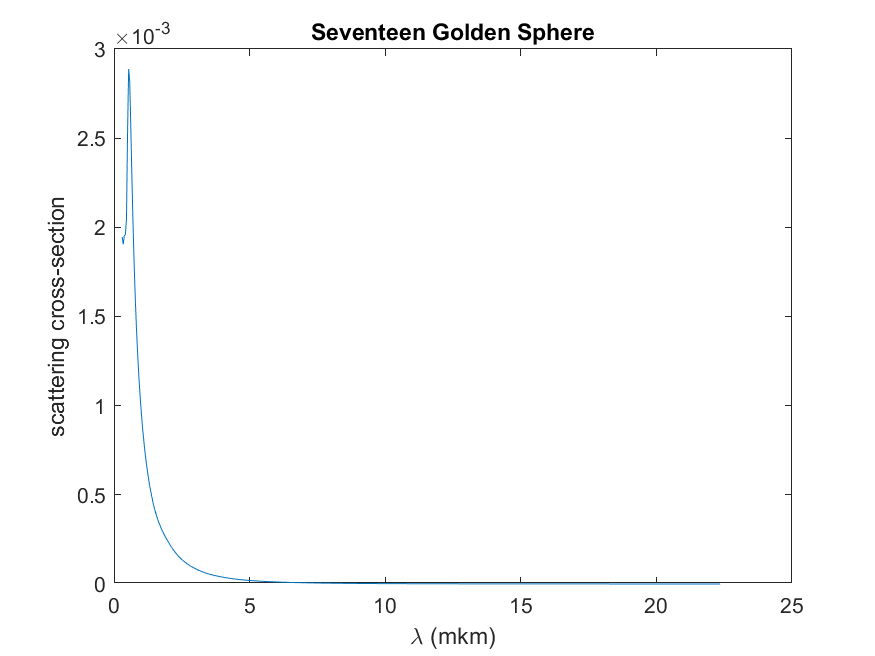
\includegraphics[width=0.5\linewidth]{seventeenGoldSphereCrossSection}
	\caption{Рассеяние на 17 золотых сферах}
	\label{fig:seventeenGoldSphereCrossSection}
\end{figure}
\begin{figure}[h!]
	\centering
	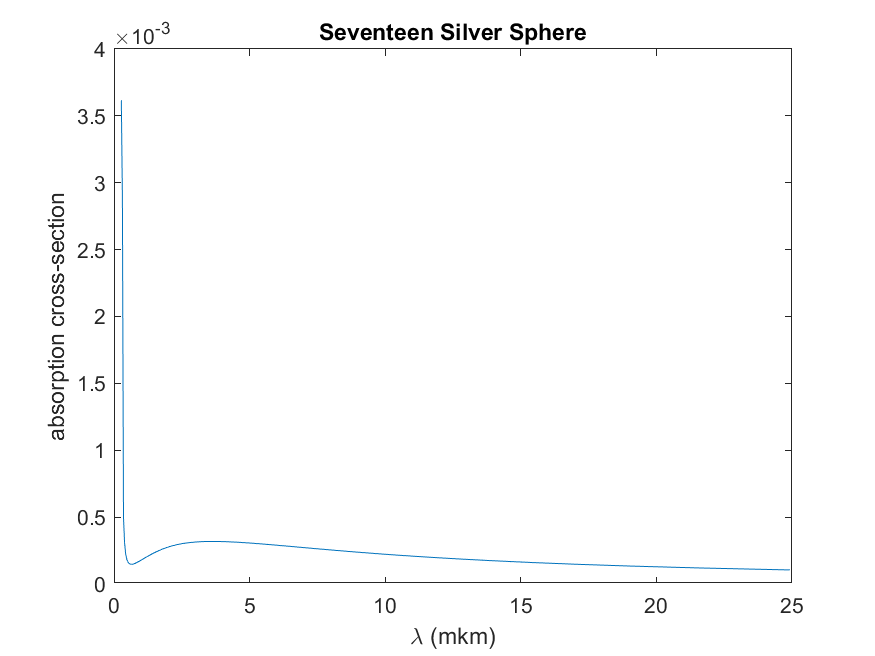
\includegraphics[width=0.5\linewidth]{seventeenSilverSphereAbsorptionSection}
	\caption{Поглощение на 17 серебряных сферах}
	\label{fig:seventeenSilverSphereAbsorptionSection}
\end{figure} 
\begin{figure}[h!]
	\centering
	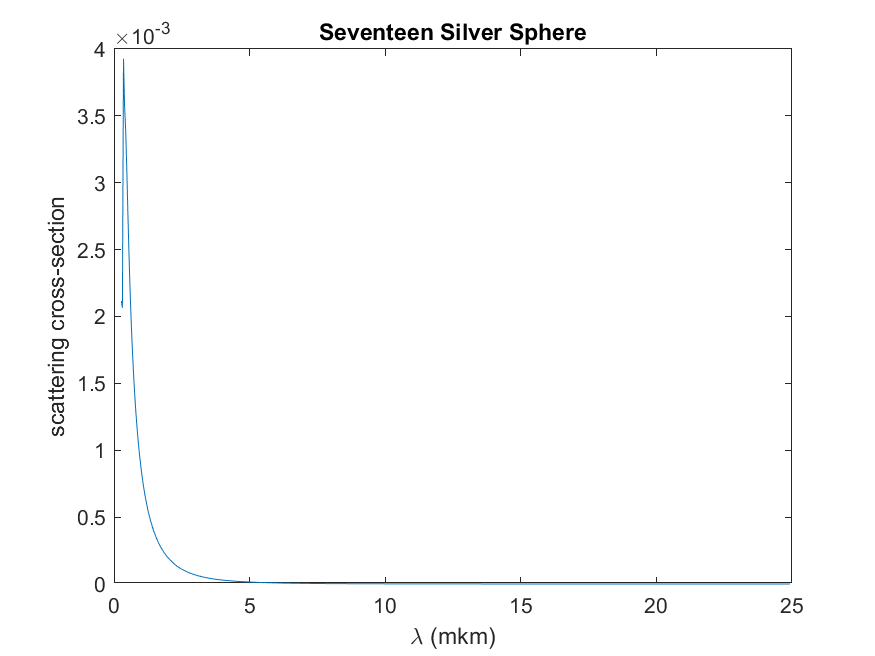
\includegraphics[width=0.5\linewidth]{seventeenSilverSphereCrossSection}
	\caption{Рассеяние на 17 серебряных сферах}
	\label{fig:seventeenSilverSphereCrossSection}
\end{figure} \\